% See http://tex.stackexchange.com/questions/168169/options-for-supplementary-materials-in-preprint-version-revtex-arxiv

\pagebreak
\begin{center}
\textbf{\large Supplemental Materials}
\end{center}

\setcounter{equation}{0}
\setcounter{figure}{0}
\setcounter{table}{0}
% \setcounter{page}{1}
\makeatletter
\renewcommand{\theequation}{S\arabic{equation}}
\renewcommand{\thefigure}{S\arabic{figure}}
% \renewcommand{\bibnumfmt}[1]{[S#1]}
% \renewcommand{\citenumfont}[1]{S#1}

Data and notebooks for these analyses are available at \url{https://github.com/hammerlab/XXX}

\begin{figure}
\centering
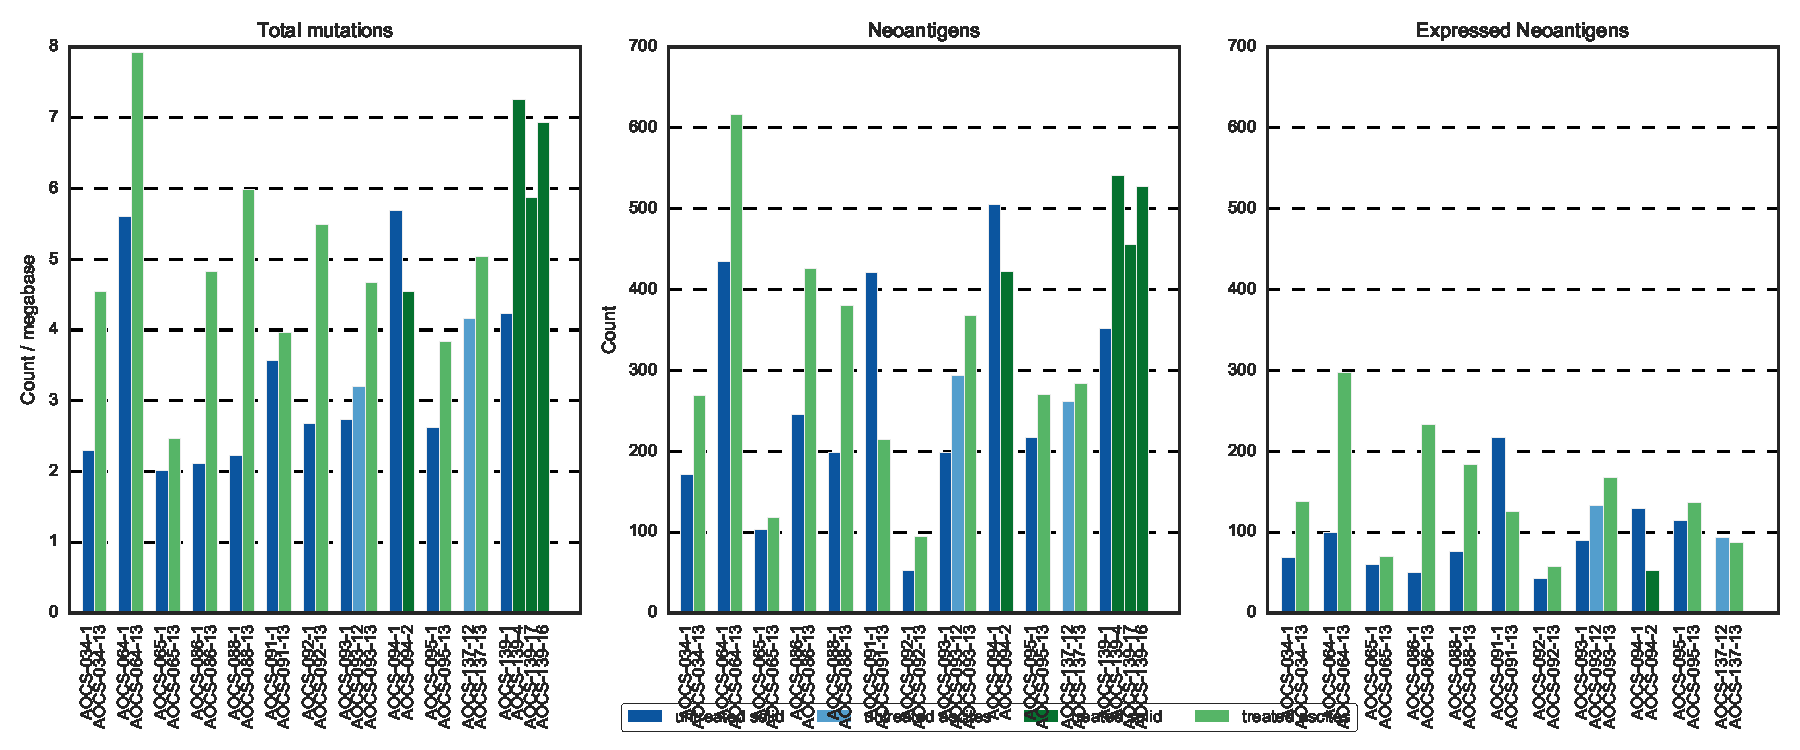
\includegraphics[scale=1.0]{figures/paired_counts.pdf}
\caption{Mutations, neoantigens, and expressed neoantigens for the donors with paired pre-/post-chemotherapy samples.}
\label{sfig:supp_paired}
\end{figure}

\begin{figure}[htbp]
\centering
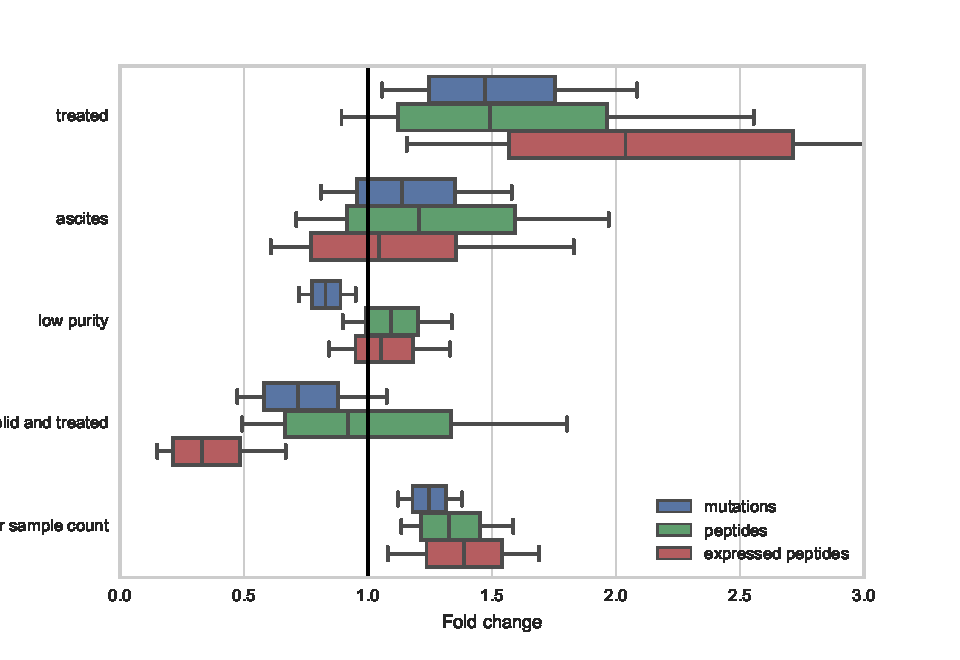
\includegraphics[scale=1.0]{figures/bayesian_model_effects.pdf}
\caption{Bayesian model effects. }
\label{fig:bayesian_model_effects}
\end{figure}

\begin{figure}
\centering
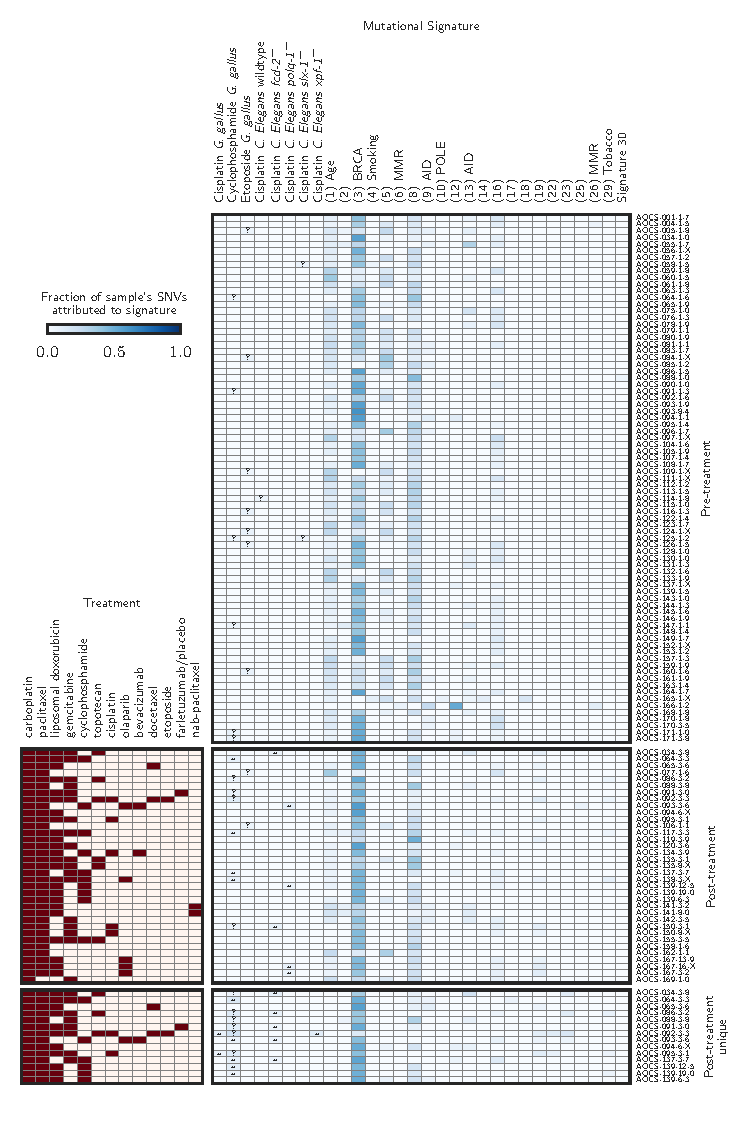
\includegraphics[scale=1.0]{figures/supplementary_signatures.pdf}
\caption{\textbf{Mutational signature deconvolutions for all samples.} See main text figure~\ref{fig:signatures} for more information.}
\label{sfig:supp_signatures}
\end{figure}

\begin{figure}
\centering
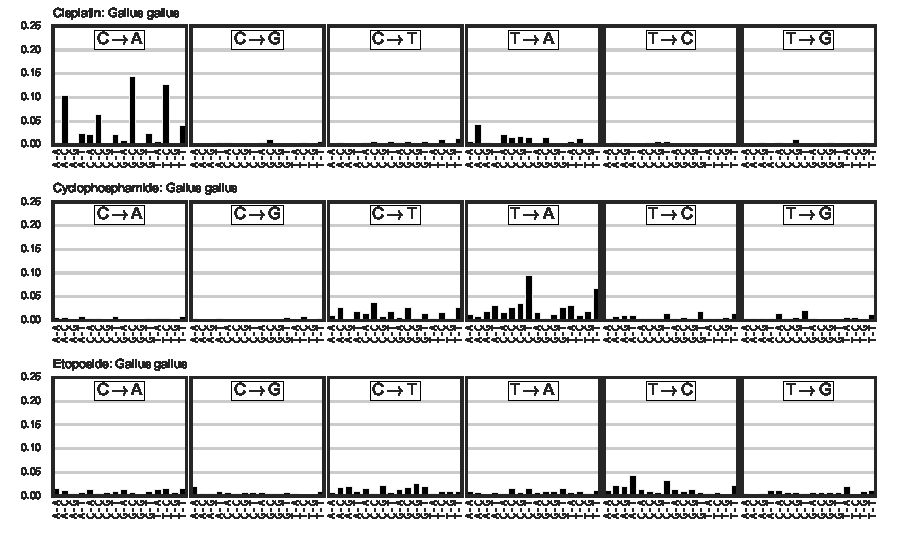
\includegraphics[scale=1.0]{figures/extracted_signatures_chicken.pdf}
\caption{Mutational signatures extracted from \cite{Szikriszt_2016}}
\label{sfig:supp_extracted_signatures_chicken}
\end{figure}

\begin{figure}
\centering
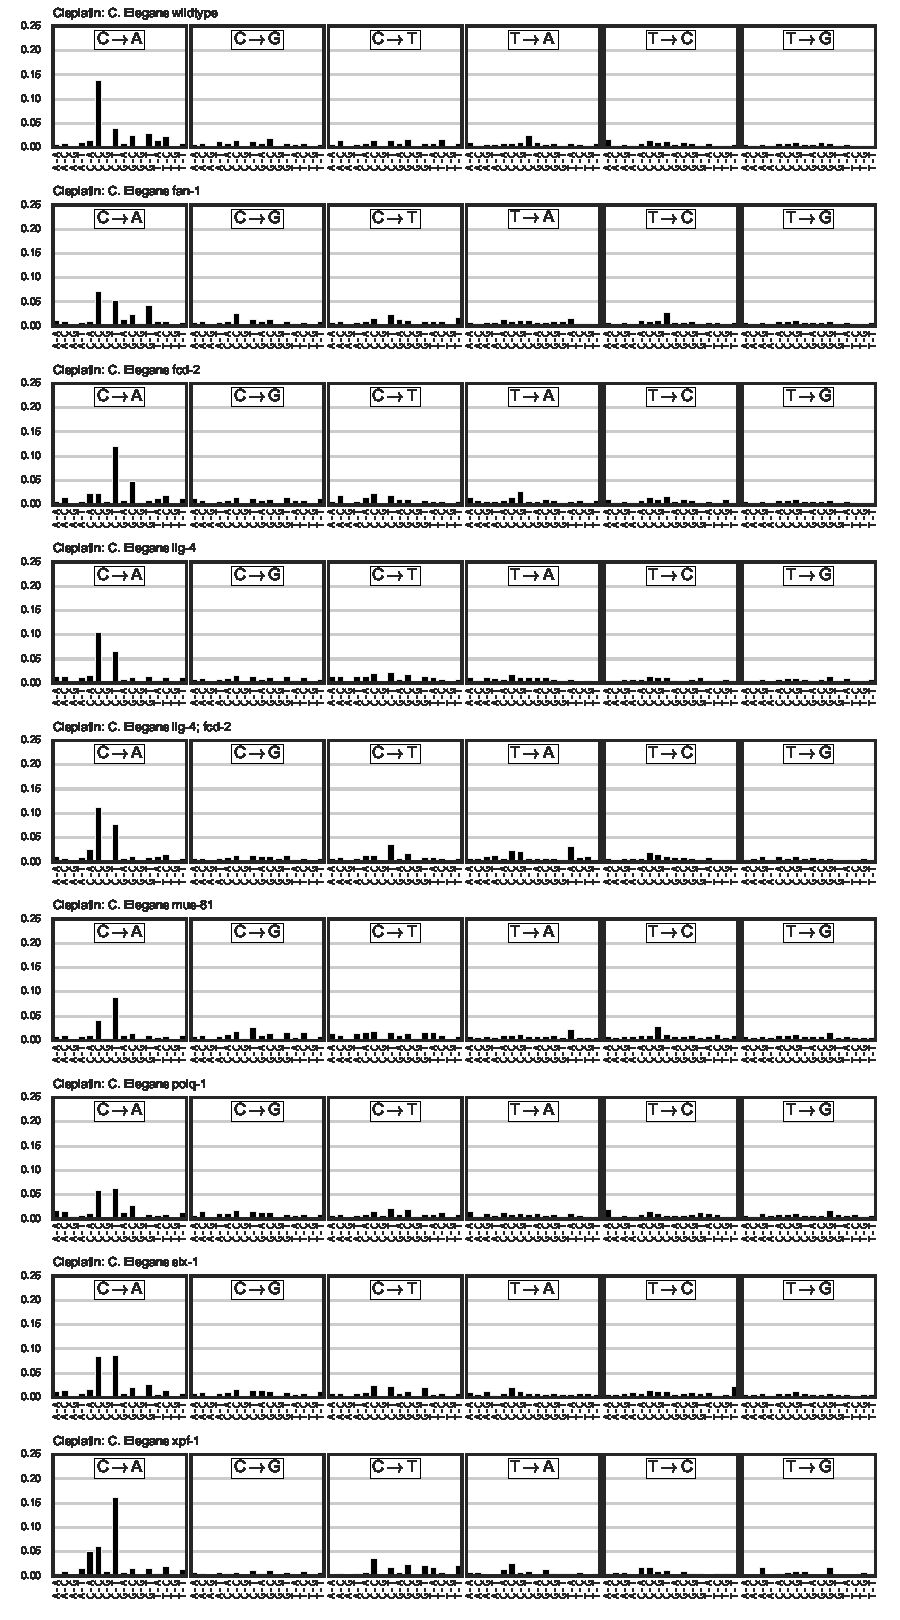
\includegraphics[scale=1.0]{figures/extracted_signatures_worm.pdf}
\caption{Mutational signatures extracted from \cite{Meier_2014}}
\label{sfig:supp_extracted_signatures_worm}
\end{figure}

\FloatBarrier
